	\section{Interfaz 1.00 Pantalla de inicio.} \label{inter:interfaz01}
	\subsection{Descripción de la pantalla}
Todos los elementos se encuentran centrados en esta pantalla. En la parte centro superior se encuentra el logotipo del juego. Abajo de éste, se puede leer el mensaje: "Toque la pantalla para empezar". Al pie de la pantalla se puede ubica la información de derechos de autor del juego.
	\subsection{Estados del juego}
Es el estado inicial del juego.
Al tocar la pantalla se muestra la Interfaz 2.0 (ver apartado \ref{inter:interfaz02}).
	\subsection{Imagen}
\begin{figure}
  \centering
   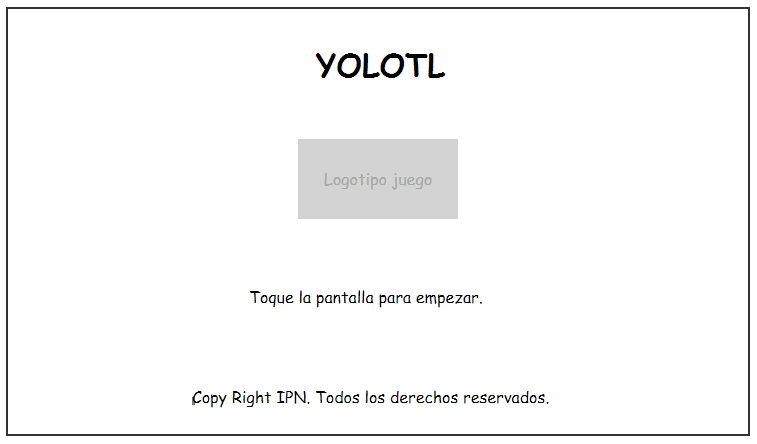
\includegraphics[width=0.6 \textwidth]{Imagenes/interfaz00}
  \caption{Interfaz 1.0 Pantalla de inicio.}
  \label{fig:PInicio}
\end{figure} 

Ver figura \ref{fig:PInicio}
